\documentclass[abstract=on,twoside,10pt,a4paper,bibliography=totocnumbered]{report}
\usepackage[paper=a4paper,left=25mm,right=25mm,top=25mm,bottom=30mm]{geometry}
\usepackage[doublespacing]{setspace}
\usepackage[english]{babel}
% \usepackage[utf8]{inputenc}
\usepackage[default]{lato}
\usepackage[T1]{fontenc}
\usepackage{amsmath}
\usepackage{colortbl}
\usepackage{amsfonts}
\usepackage{amssymb}
\usepackage{gensymb}
\usepackage{textcomp}
\usepackage{graphicx}
\usepackage{tikz}
\usepackage{enumerate}
\usepackage{enumitem}
\usepackage{subcaption}
\usepackage{booktabs}
\usepackage[hidelinks]{hyperref}
% \usepackage{hyperref}
\usepackage[nameinlink]{cleveref}
\usepackage{multirow}
\usepackage{arydshln}
\usepackage[flushleft]{threeparttable}
\usepackage{scalerel}
\usepackage{makecell}
\usepackage{ifthen}
\usepackage{tikz}
\usepackage{lineno}
\usepackage{subfiles}
\usepackage{pdfpages}
\usepackage{adjustbox}
% \usepackage{parskip}
\usepackage{fancyhdr}
\usepackage[all]{nowidow}
\usepackage[titletoc]{appendix}
\usepackage[explicit]{titlesec}
\usepackage[nottoc,notlot,notlof]{tocbibind}
\usetikzlibrary{svg.path}

%------------------------------------------------------------------------------
%  Bibtex vs Biblatex
%------------------------------------------------------------------------------
% While bibtex is very nice to use, it's insanely slow. I therefore work with
% bibtex until the final stage. Set the value below to "true" or "false" to pick
% which one should be used.
\newboolean{usebiblatex}
\setboolean{usebiblatex}{true}

% We also load our custom preamble (stored in "FinalThesis.sty")
\usepackage{FinalThesis}

%------------------------------------------------------------------------------
%  MAIN DOCUMENT
%------------------------------------------------------------------------------
\begin{document}

% Rename bibliography (Biber)
\renewcommand{\bibname}{References}

% Change page numbering
\pagenumbering{gobble}

% Titlepage and Preamble
\subfile{Titlepage/TitlepageGerman}

% Add linenumbers
% \linenumbers

\chapter*{Summary}

Connectivity is a crucial prerequisite for animals to move and disperse, which
in turn promotes genetic exchange, facilitates range-shifts, and enables the
recolonization of vacant habitats. Preserving and establishing movement
corridors that enhance connectivity and facilitate dispersal have therefore
become tasks of utmost importance in conservation science. Nevertheless, many of
the methods employed to study dispersal and connectivity suffer from important
limitations that inhibit a more holistic understanding of landscape
connectivity. In this doctoral thesis, I investigate various aspects of animal
dispersal and landscape connectivity, focusing on several of these limitations.
Specifically, I propose a novel method for quantifying landscape connectivity,
examine the impact of changing environmental conditions due to climate change,
and investigate the role of seasonal factors when modeling connectivity. I also
present and compare multiple methods for dealing with temporally irregular data
when estimating habitat and movement preferences of dispersers from GPS data.
These aspects are researched primarily using dispersing African wild dogs from
northern Botswana as a study system. Due to the study species' wide-ranging
behavior and the study areas' highly seasonal habitats, the study system offers
a unique opportunity to investigate patterns of dispersal and connectivity in
light of the outlined considerations.

\Cref{GeneralIntroduction} introduces the general background and research topics
of this thesis. In particular, I discuss the importance of dispersal and
connectivity in the context of conservation science and highlight multiple
limitations in current connectivity research. I also describe the study system
and give a brief overview of the data collection and general research methods.

\Cref{ChapterSimulation} introduces a novel and simple workflow for examining
landscape connectivity using simulations from individual-based movement models.
To date, connectivity is primarily investigated using least-cost path models or
circuit theory. However, both approaches require highly subjective permeability
surfaces as inputs and make unreasonable assumptions that are rarely met by
dispersing individuals. The proposed simulation workflow overcomes these
shortcomings and provides a powerful alternative for studying connectivity via
simulated dispersal trajectories and a complementary set of connectivity
metrics. I exemplify the application of the proposed workflow and assess
connectivity for dispersing wild dogs in the Kavango-Zambezi Transfrontier
Conservation Area, revealing major movement corridors and highlighting dispersal
hotspots. This chapter was published in \textit{Landscape Ecology} in 2023
(\url{https://doi.org/10.1007/s10980-023-01602-4}).

\Cref{ChapterFlood} investigates how changing environmental conditions due to
climate change affect on-the-ground conditions and, ultimately, species'
ability to disperse. Specifically, I investigate how changes in the flooding
regime of the Okavango Delta impact wild dogs' ability to disperse between
adjacent regions. For this, I combine the simulation framework from
\Cref{ChapterSimulation} with long-term remote sensing data of the Delta's flood
extent and simulate dispersal under an increased and a reduced flood scenario.
Both scenarios represent conceivable outcomes under the impact of climate
change. I show that an increased flood reduces connectivity and prolongs
dispersal durations, yet that the opposite is true under a reduced flood.
Importantly, I highlight that the likely hotspots for human-wildlife conflict
shift depending on future flood conditions. This chapter was published in
\textit{Global Change Biology} in 2024
(\url{https://doi.org/10.1111/gcb.17299}).

\Cref{ChapterSeasonality} conceptually motivates that seasonality can enter
connectivity analyses at three distinct modeling stages, resulting in multiple
configurations that greatly differ in terms of the dynamism they encapsulate. To
test whether the incorporation of seasonality into connectivity analyses
improves their predictive ability, I fit the models associated with each
configuration and employ a rigorous validation procedure that compares predicted
with observed movement. I also demonstrate that the simulation workflow
presented in previous chapters can accommodate for a previously unseen degree of
seasonality by allowing the landscape to change as the simulated dispersers
move. Surprisingly, I find that predictions from the fitted models only
marginally improve upon increasing the degree of seasonality. Nevertheless,
inferred patterns of connectivity differ, with connectivity being more evenly
distributed when seasonality is accounted for.

\Cref{ChapterIrregularity} revisits the statistical framework of integrated
step-selection functions, which are frequently employed in connectivity studies
to assess habitat preferences from GPS data. Currently, step-selection functions
require temporally regularly spaced GPS data, which implies that irregular data
need to be removed. This can result in a substantial loss of data, especially in
studies where data are already scarce. Hence, I propose and compare several
methods for dealing with irregular data, thereby allowing to retain additional
data for modeling. I compare different methods using simulated data with known
parameters and show that retaining irregular data can aid to reduce model
uncertainty if appropriate methods are employed. Finally, I exemplify the
application of the best performing method using GPS data collected on a spotted
hyena from northern Botswana. The use of hyena data instead of wild dog data was
mainly due to the availability of an extensive dataset on a single spotted
hyena. This chapter was published in \textit{Movement Ecology} in 2024
(\url{https://doi.org/10.1186/s40462-024-00476-8}).

Finally, in \Cref{GeneralDiscussion}, I summarize my findings and embed them in
a broader context. I also provide an outlook for topics that require further
research, and provide conservation insights for the African wild dog.

Overall, this thesis provides a detailed investigation of dispersal and
connectivity for the endangered African wild dog and propose several novel
methods and approaches. It thereby challenges established practices and suggests
new avenues to model dispersal movements. By combining methodological novelty
with conservation insights, this thesis not only advances our understanding of
connectivity in general, but yields specific insights that facilitate the
implementation of targeted conservation measures. The dispersal model refined
throughout the chapters furthermore sets the foundation for a comprehensive
population viability analysis that realistically captures how dispersers move
across the landscape.

\newpage

% Table of content
\begin{onehalfspacing}
\pagestyle{empty}
\tableofcontents
\end{onehalfspacing}
\newpage

% Set up fancy header
\pagestyle{fancy}
\fancyhf{}
\fancyhead[LO]{\rightmark}
\fancyhead[RO]{\thepage}
\fancyhead[RE]{\rightmark}
\fancyhead[LE]{\thepage}

% General Introduction
\includepdf{Images/Delta.jpg}
\pagenumbering{arabic}
\subfile{Chapter_00/Manuscript}

% Chapter 1 - Three-Step Approach
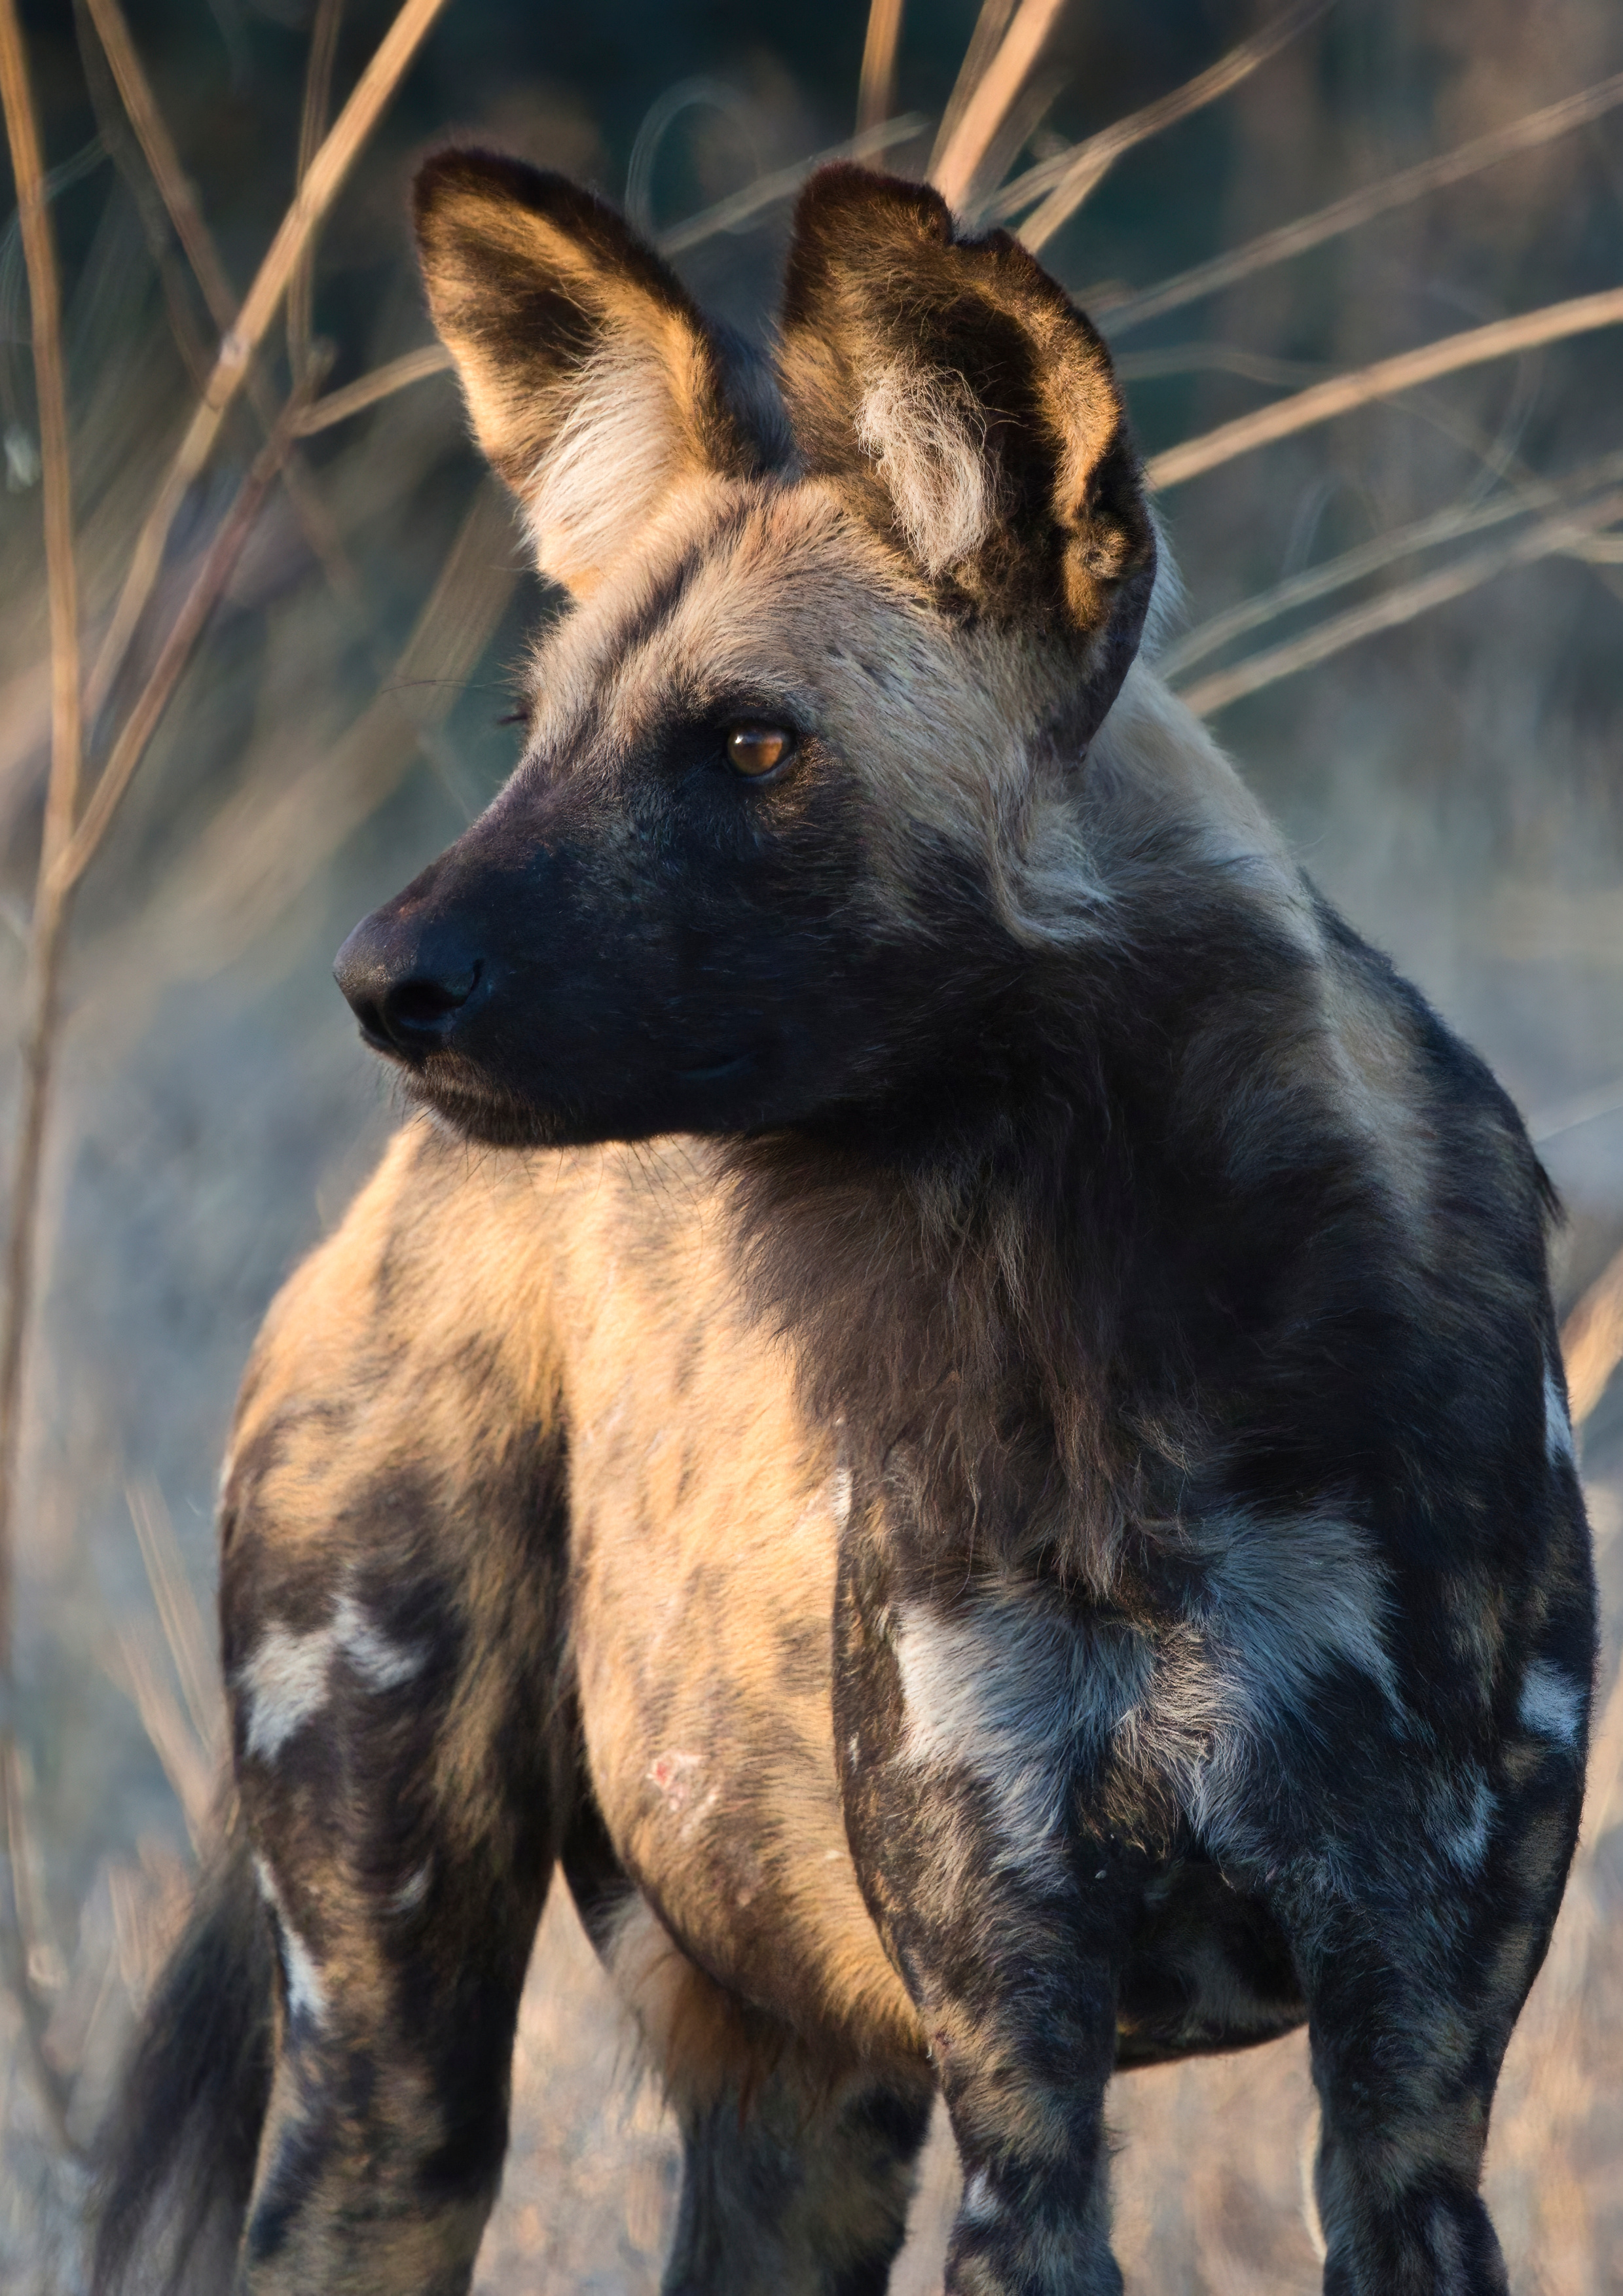
\includepdf{Images/Jessie.jpg}
\subfile{Chapter_01/Manuscript}
\begin{subappendices}
\subfile{Chapter_01/Manuscript_Support}
\end{subappendices}

% Chapter 2 - Extreme Flooding
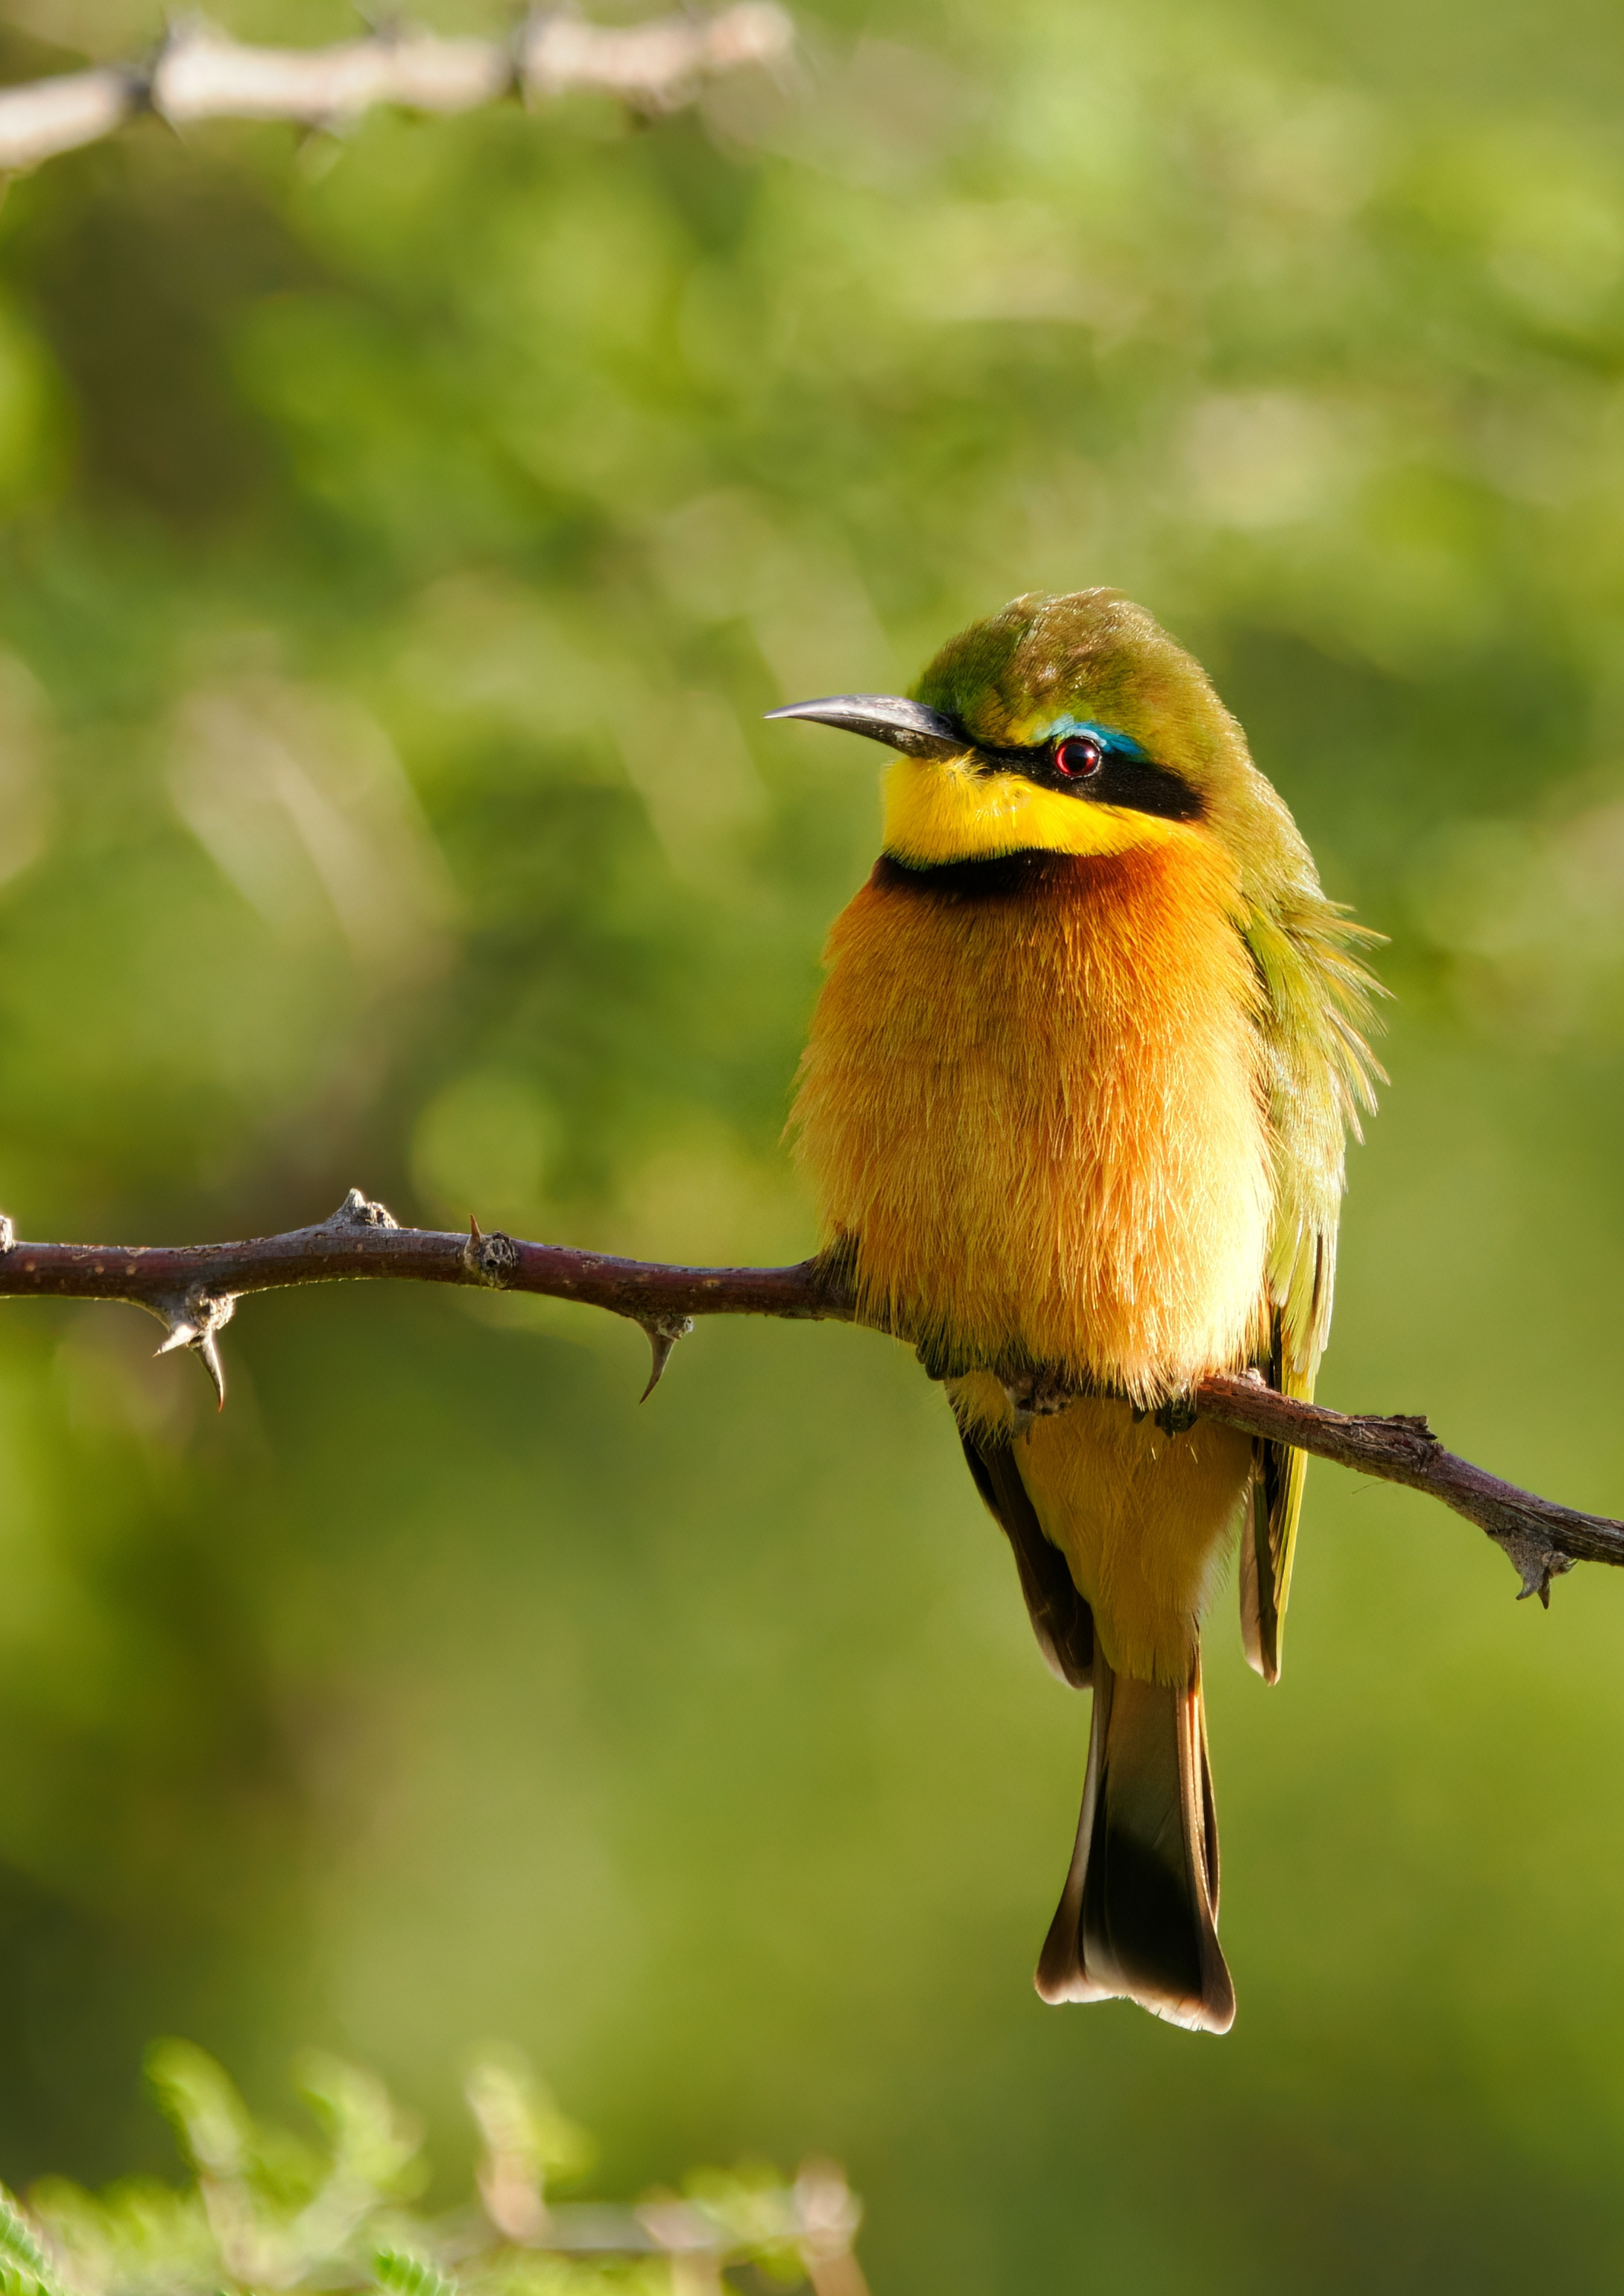
\includepdf{Images/BeeEater.jpg}
\subfile{Chapter_02/Manuscript}
\begin{subappendices}
\subfile{Chapter_02/Manuscript_Support}
\end{subappendices}

% Chapter 3 - Seasonality
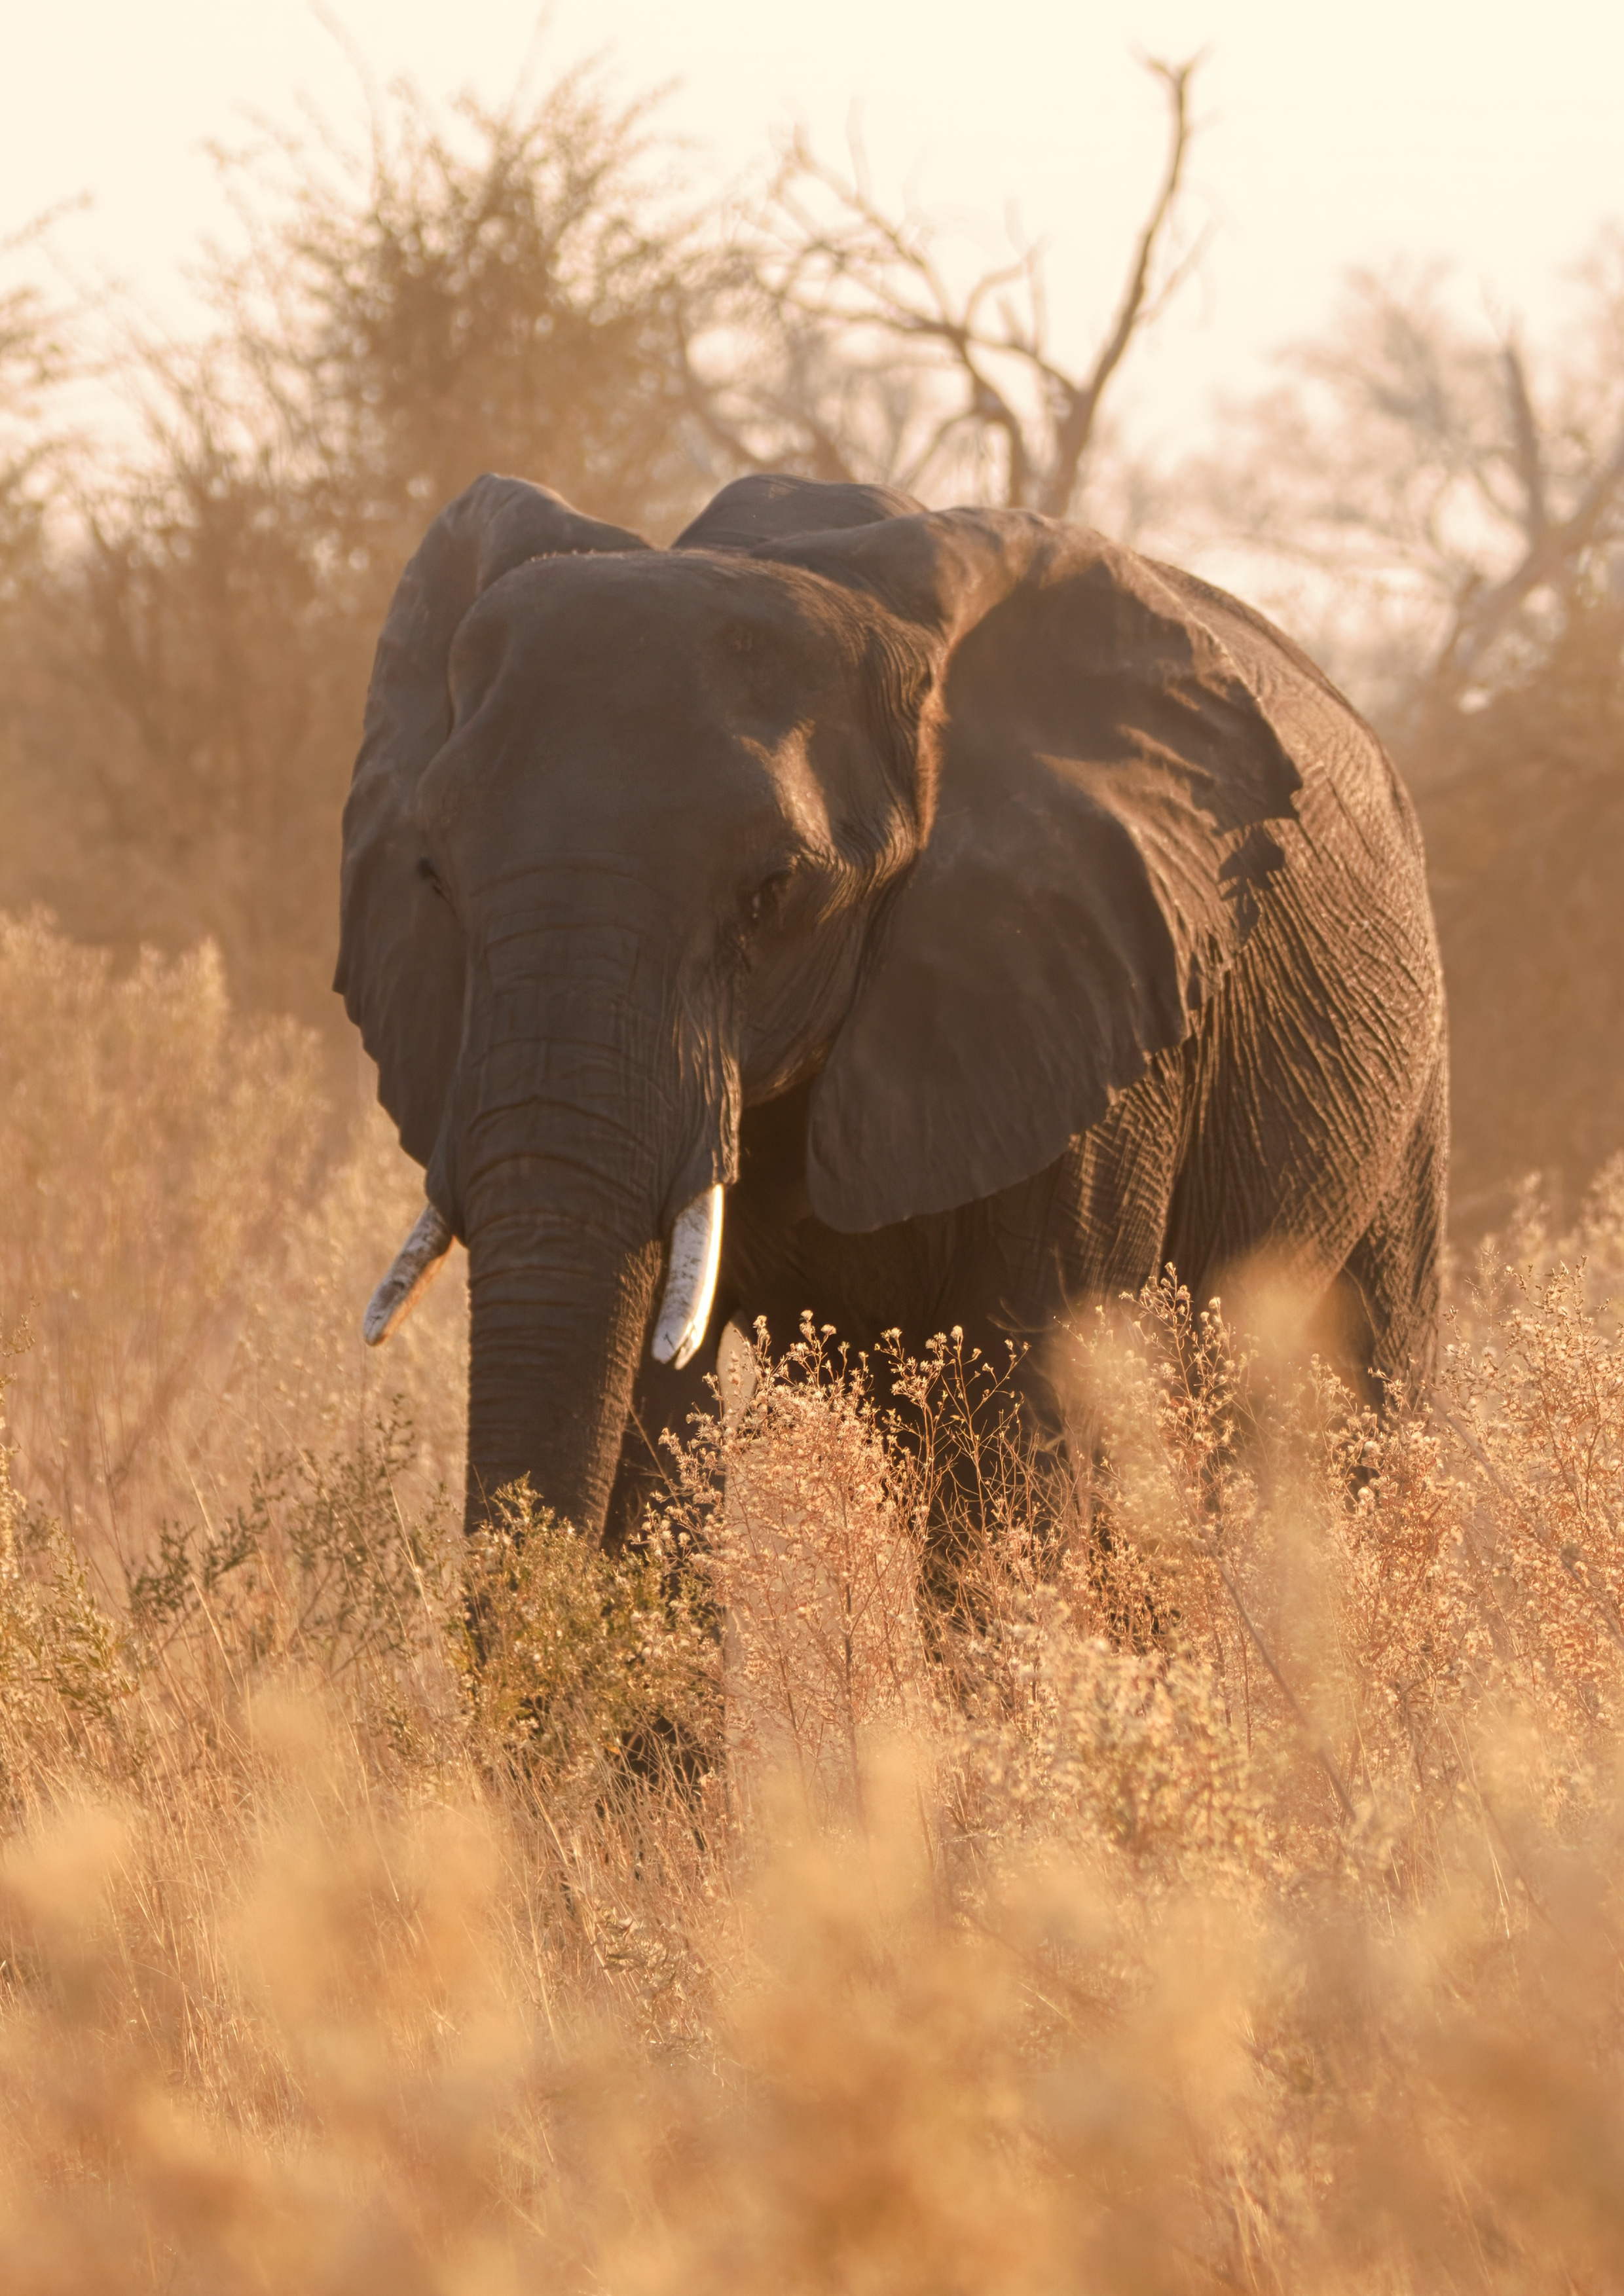
\includepdf{Images/Elephant.jpg}
\subfile{Chapter_03/Manuscript}
\begin{subappendices}
\subfile{Chapter_03/Manuscript_Support}
\end{subappendices}

% Chapter 4 - Irregular iSSFs
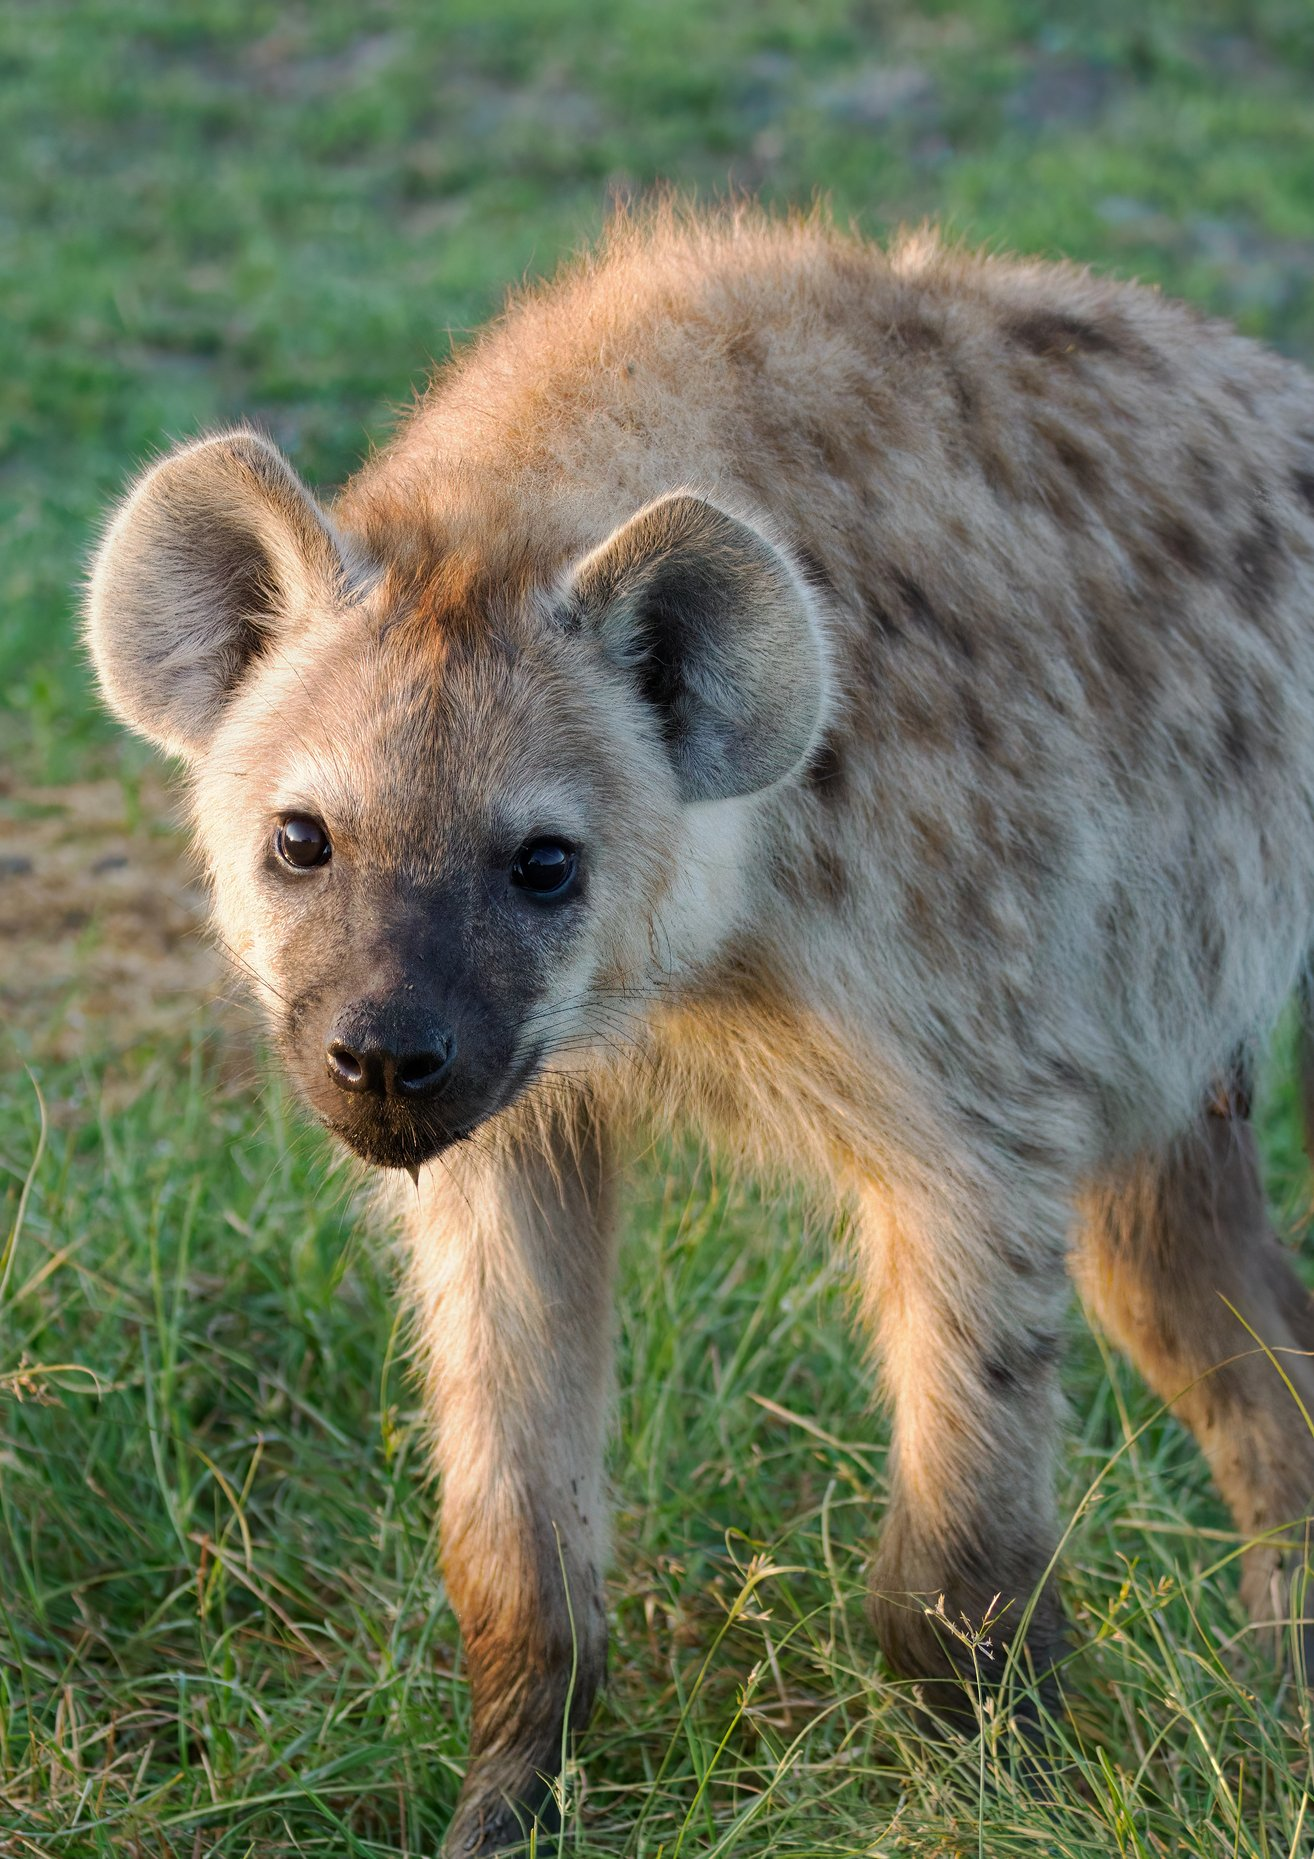
\includepdf{Images/Hyena.jpg}
\subfile{Chapter_04/Manuscript}
\begin{subappendices}
\subfile{Chapter_04/Manuscript_Support}
\end{subappendices}

% Chapter 5 - General Discussion
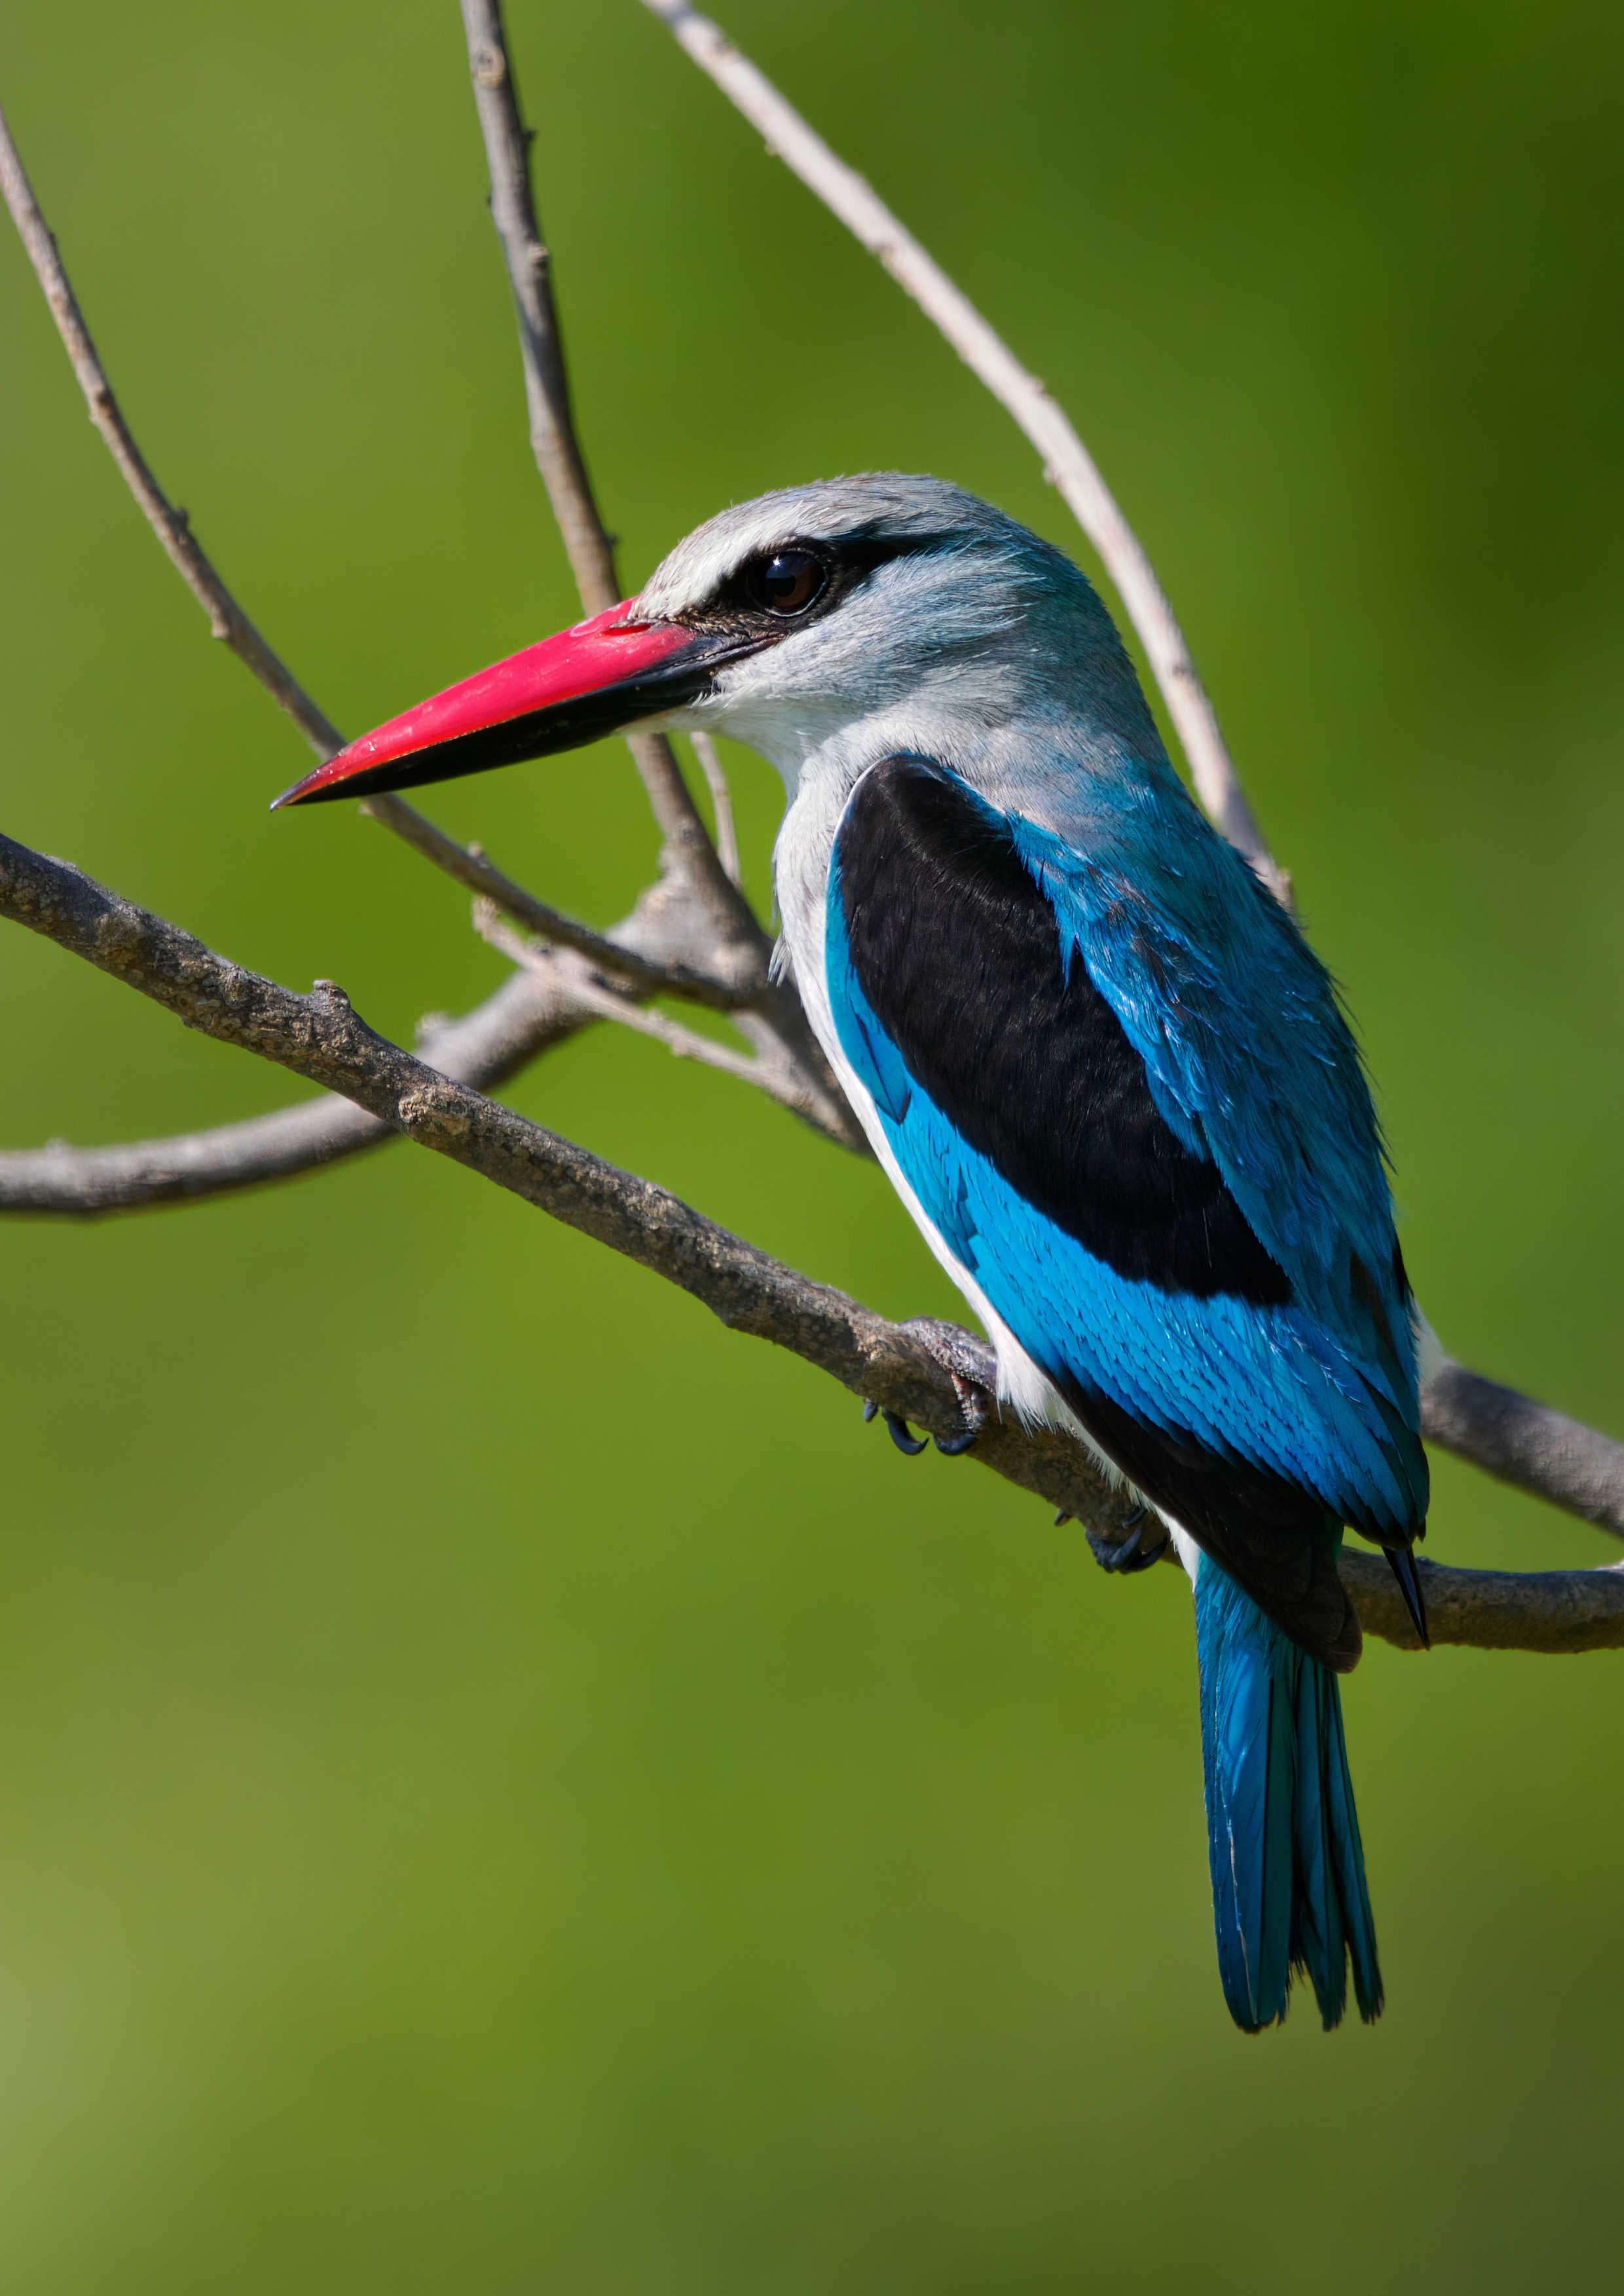
\includepdf{Images/Kingfisher.jpg}
\subfile{Chapter_05/Manuscript}

% Acknowledgements
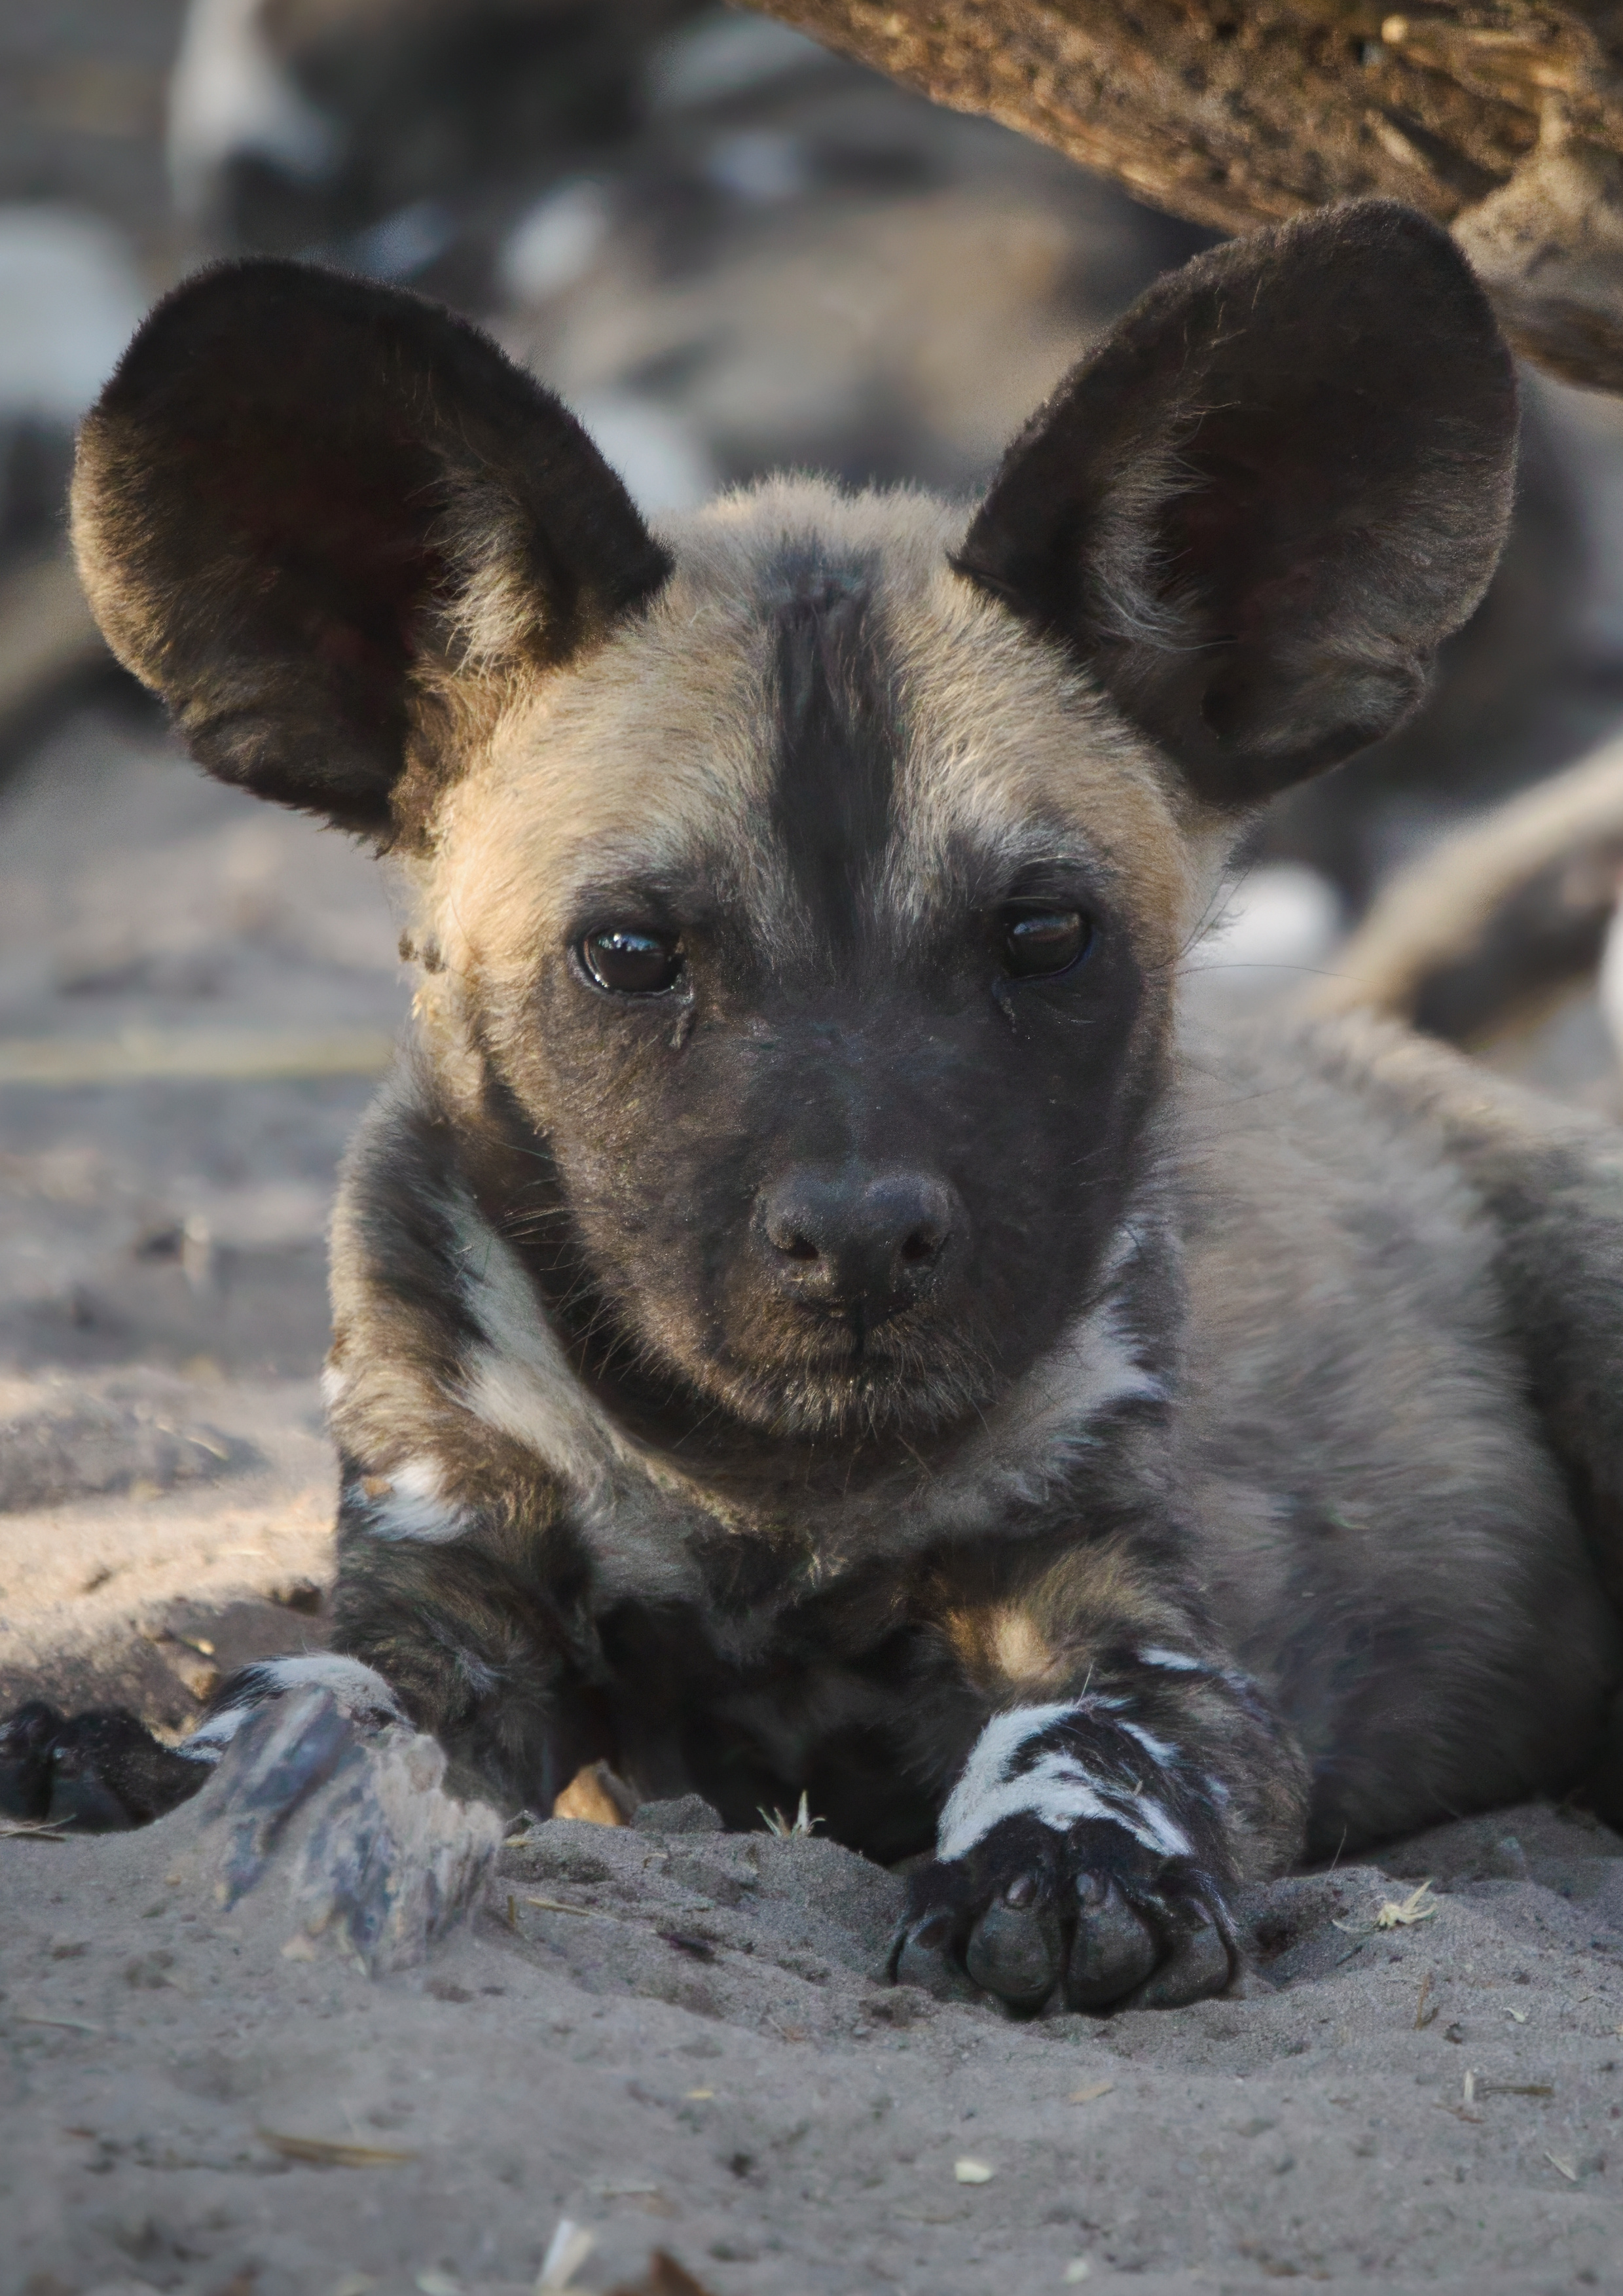
\includepdf{Images/WildDogPup.jpg}
\subfile{Acknowledgements/Manuscript}

% Appendix: Additional Works
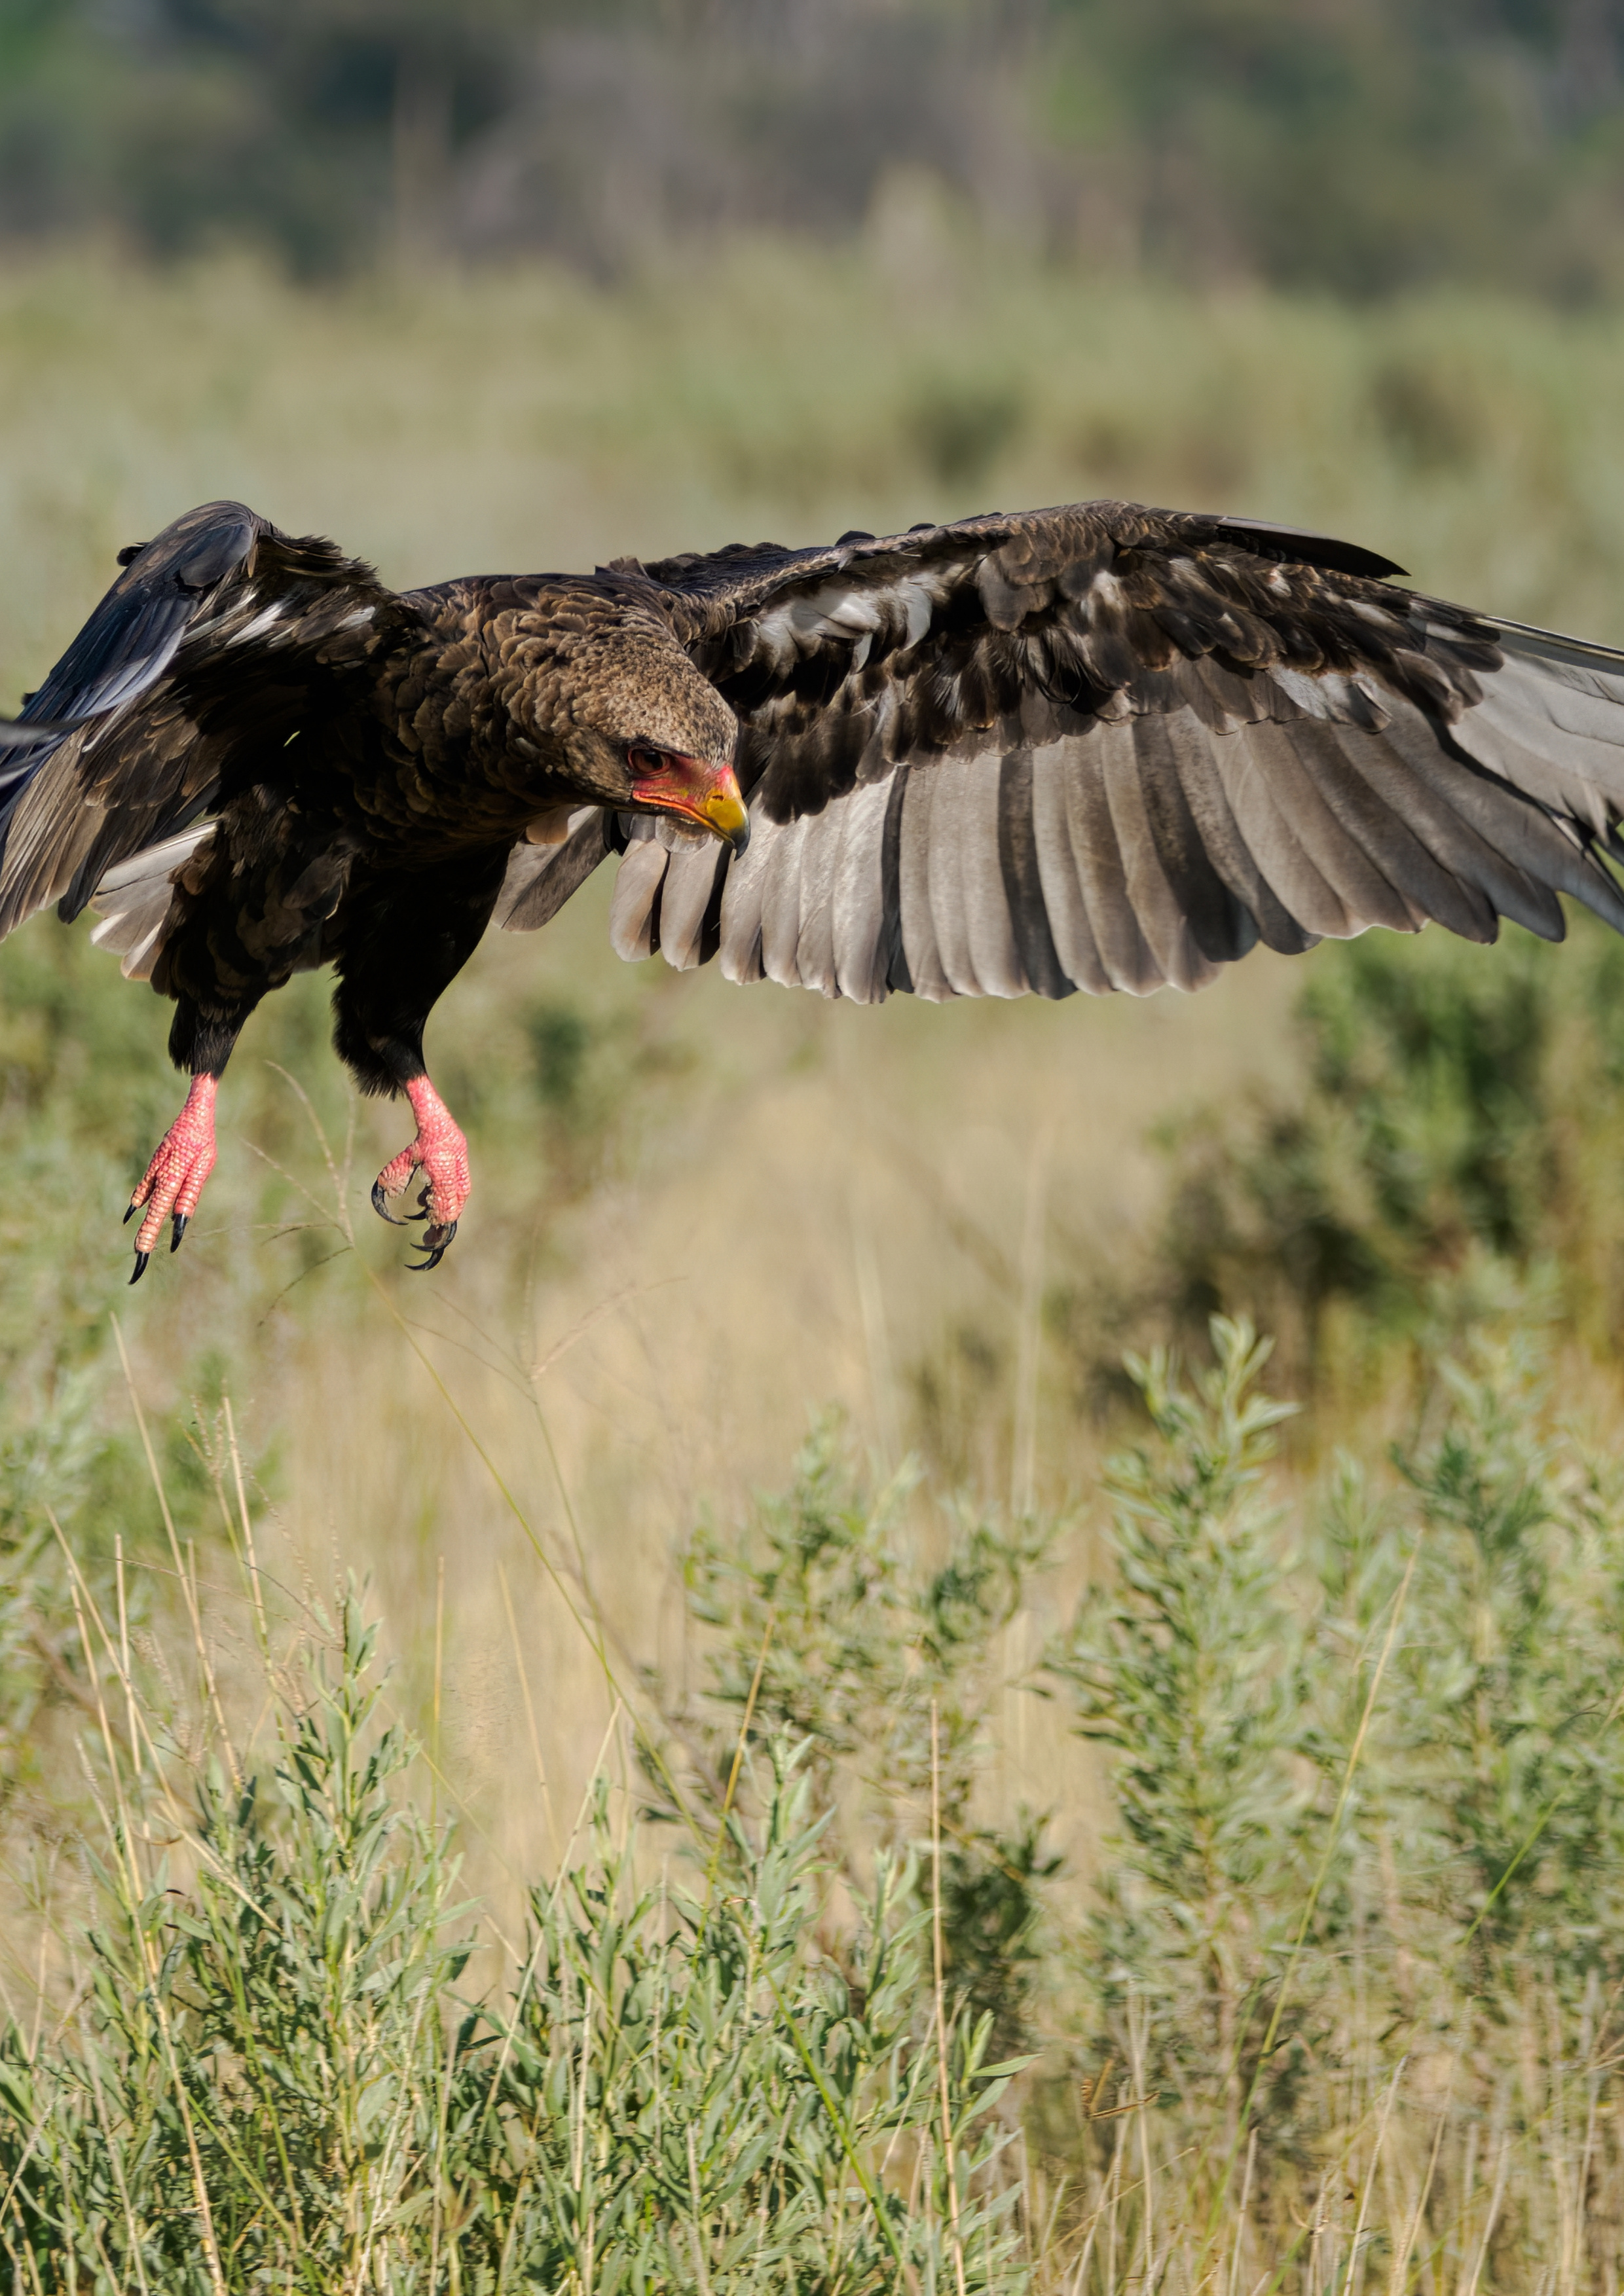
\includepdf{Images/Bateleur.jpg}
\begin{appendices}
\subfile{Appendix/Manuscript}
\end{appendices}

%------------------------------------------------------------------------------
%  Bibliography
%------------------------------------------------------------------------------
% Depending on whether we're using bibtex or biblatex, a different snippet is
% used
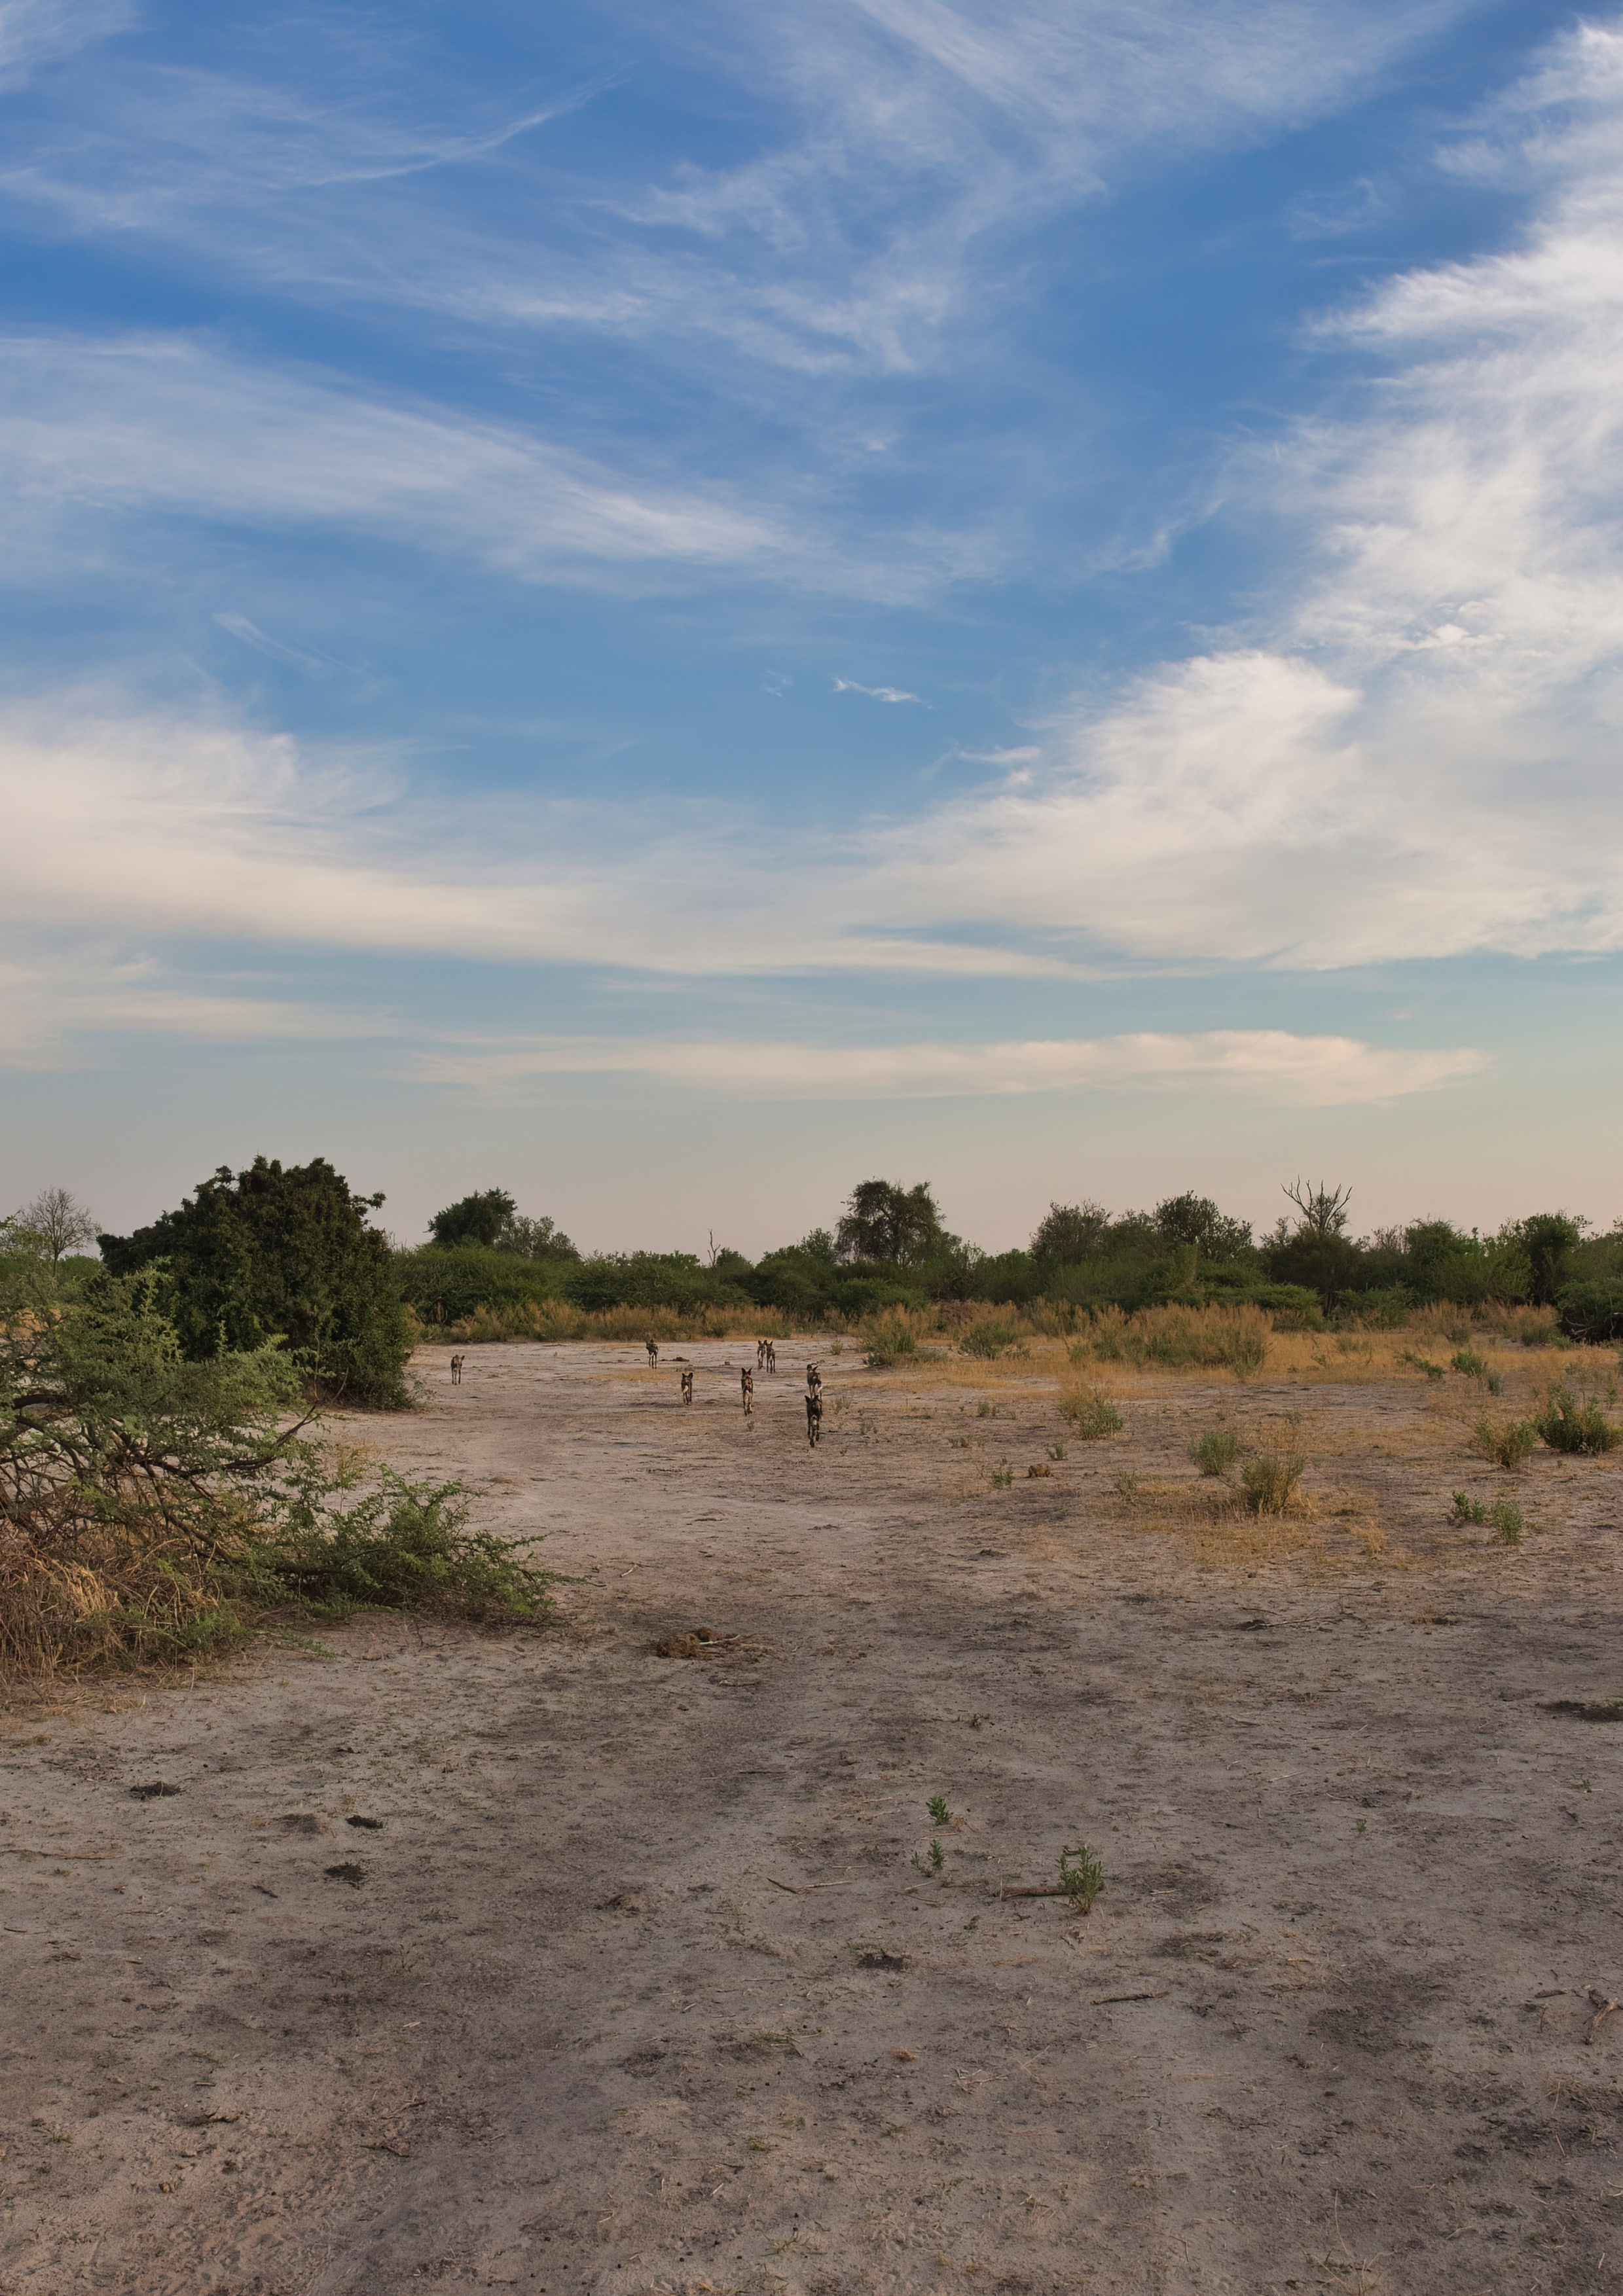
\includepdf{Images/DogFollow.jpg}
\newpage
\begin{singlespacing}
\ifthenelse{\boolean{usebiblatex}}{
  \begin{refcontext}[sorting=nyt]
  \printbibliography[title=References,heading=bibintoc]
  \end{refcontext}
}{
  \bibliography{\subfix{LiteratureBibtex.bib}}
}
\end{singlespacing}

\end{document}
